\begin{figure}[!h]
\caption{PC use by job type}
\subfloat[Below GCSE C]{\includegraphics[width=.5\textwidth]{../output/pcuse1}} \subfloat[GCSE C-A levels]{\includegraphics[width=.5\textwidth]{../output/pcuse2}} \\ \subfloat[Bachelor+]{\includegraphics[width=.5\textwidth]{../output/pcuse3}} \subfloat[Below GCSE C/GCSE C-A levels]{\includegraphics[width=.5\textwidth]{../output/pcuse12}} \\ \subfloat[GCSE C-A levels/Bachelor+]{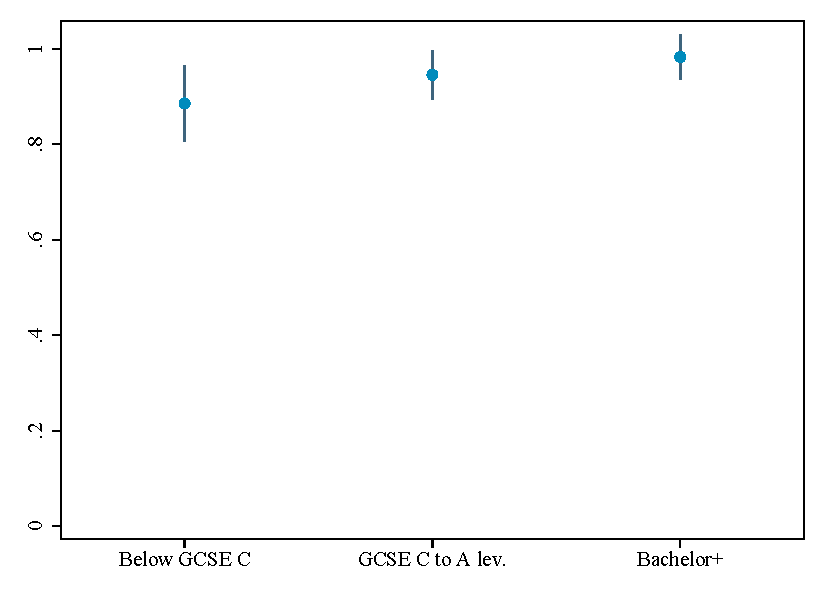
\includegraphics[width=.5\textwidth]{../output/pcuse23}} 
\par \begin{minipage}[h]{\textwidth}{\scriptsize\textbf{Note:} graphs show regression coefficients. Dependent variable is a dummy variable equal to 1 if a pc is used. Regressions include occupation and year fixed-effects. CI based on robust standard errors. Higher values indicate less complex pc use. Figure generated on 12 Jun 2020 at 15:40:41. Figure generated using the dofile 3\_sesAnalysis/pcUseTables.do.}\end{minipage}
\end{figure}
